\chapter{Introduction}
\label{sec:level1}

\section{Fission and Neutron Correlations}
The photofission reaction occurs during the de-excitation of a nucleus after the absorption of a photon.
For photon energies between 6 and 25 MeV, this absorption occurs primarily via the giant dipole resonance (GDR).
One distinct and useful aspect of photofission, particularly when compared to neutron-induced fission, is the simple set of selection rules for the transfer of angular momentum.
In photofission, there is a relatively low transfer of angular momentum to the nucleus, and as a result photon absorption occurs primarily via E1 absorption and to a lesser extent E2 absorption.
Because of this selectivity, photofission is commonly used as a means to study sub-nuclear structures and the fundamentals of the fission process.
For even-even nuclei, $J^{\pi}$ values of the excited state are restricted to the electric dipole ($1^{-}$) and electric quadrupole ($2^{+}$) states, which gives rise to anisotropies in the fission fragment angular distribution that are far more pronounced than for other types of fission~\cite{1977FragAss}.
Detailed studies of the dynamics of fission provide significant insight into the fundamental physics of this process, and have the potential to shed light on model parameters needed for a comprehensive theoretical description of fission.
Fission neutron emission can be classified into two categories, depending on the time of emission: delayed and prompt.
Delayed neutrons account for only $\sim1\%$ of total neutron emission in actinide photofission~\cite{Caldwell2017DelayedNs}.
Delayed neutrons are not important to this study, and this measurement is insensitive to them because they are emitted milliseconds after fission.
Prompt fission neutrons are defined as neutrons that are emitted either immediately after ($<10^{-14}$ seconds) fission or during the scission of the nucleus, and account for the remaining $\sim99\%$ of neutron emission~\cite{Caldwell2017DelayedNs}.
Prompt fission neutron production occurs by means of two distinct mechanisms.
The dominant mechanism is neutron emission from the fully accelerated fragments.
The second mechanism, referred to as \textit{early} or \textit{scission} neutron emission, is the emission of neutrons during either the scission of the nucleus, or the acceleration of the fission fragments.
Both cases are described below.

A large number of past studies have established that the majority of prompt fission neutrons (80\%--98\%) are emitted from the fully accelerated fragments, while the remaining 2\%--20\% percent are scission neutrons~\cite{Scission2005}.
The nature of scission neutrons has remained elusive since their first tentative observation in 1962 by Bowman \emph{et al.}~\cite{Bowman}.
Models of prompt neutron emission in binary fission are based mainly on observations of neutron angular distributions relative to the fission axis, the axis along which the fragments travel in the center of momentum frame.
Another observational input for prompt neutron modeling is the neutron-neutron opening angle distribution of correlated neutron pairs, as seen in the lab frame, hereafter denoted $\theta_{nn}$.
Because fission neutrons are predominantly emitted from the fully accelerated fragments, the distribution of $\theta_{nn}$ is reflective of the underlying fundamental fission kinematics.
There are, on average, about 2 or 3 neutrons released per fission, depending on the target isotope and how the fission is induced.
It has been shown that neutrons released from the fully accelerated fission fragments are evaporated isotropically in the fragment's rest frame, and are emitted at speeds comparable to that of the fragments themselves~\cite{JORGENSEN}.
This leads to the well-known U--shaped distribution in $\theta_{nn}$, which has been reported in studies of neutron-induced, spontaneous, and, in this study, photon-induced fission.
%(see Fig.'s~\ref{fig:Cf252_us_vs_them},~\ref{fig:FinalDUResult}, and~\ref{fig:theta_abs_two_neutron}).

The U--shaped distribution of $\theta_{nn}$ can be understood as the result of the boost provided to the neutrons by the fission fragments in binary fission.
Due to the conservation of momentum, the fully accelerated fission fragments are traveling nearly back-to-back, and neutrons emitted from different fragments are boosted in opposite directions, whereas neutrons emitted from the same fragment are boosted in the same direction.
Thus, if the velocity of the fission fragments is large enough to account for a significant portion of the kinetic energy of fission neutrons, then neutron pairs emitted from the accelerated fragments will experience a favoring of opening angles near 0$^{\circ}$ (if emitted from the same fragment) and 180$^{\circ}$ (if emitted from different fragments) , and a suppression of opening angles around $90^{\circ}$.
The favoring of large and small opening angles shows a strong dependence on neutron energy, because neutrons with higher energy are more likely to have been emitted along the same direction of the fission fragments.

\section{Connection to Physics}
Two-neutron correlations in fission, and particularly photon-induced fission, are expected to shed light on several fundamental aspects of the fission process including the neutron multiplicity distributions associated with the light and heavy fission fragments, the nuclear temperatures of the fission fragments, and the mass distribution of the fission fragments as a function of energy released.
In addition, the unique kinematics of fission and the resulting two-neutron correlations have the potential to be the basis for a new tool to detect fissionable materials~\cite{Talou2018}.
Furthermore, two-neutron opening angle measurements are useful for the study of scission neutrons.
Scission neutrons are thought to be emitted isotropically in the lab frame, and so they have the effect of flattening out the U-shaped two-neutron opening angle distribution.
Because of this effect, these measurements add to the growing breadth of nuclear data needed to confirm the exact extent of the scission-neutron component in fission, which remains an open problem in nuclear physics.

\section{Past Measurements, Spontaneous and Neutron Induced Fission}
As of this writing, tabulated data for photofission is far scarcer than for neutron induced fission.
The first measurement of the angular correlation among coincident neutrons from fission was performed by Debenedetti \emph{et al.}~\cite{1948twoNCorr} in 1948 from neutron induced fission of $^{235}\text{U}$.
The next measurement of this type was performed by Pringle and Brooks in 1975~\cite{1975Cf252}, in which neutrons emitted from the spontaneous fission (SF) of $^{252}$Cf were found to have high coincidence rates at small opening angles near 0$^{\circ}$ and large opening angles near $180^{\circ}$.
In order to produce a result that is insensitive to the effects of detector geometry and efficiency, the present work uses techniques similar to reference~\cite{1975Cf252}, in which a ratio is taken between a correlated opening angle distribution and an uncorrelated opening angle distribution.
To date, numerous measurements of two-neutron angular correlation using $^{252}$Cf have been performed~\cite{Verbeke2018, Pozzi2014, 2008CF252, 1975Cf252}.
This makes $^{252}$Cf a good benchmark for two-neutron angular correlation measurements.
Fig.~\ref{fig:Cf252_us_vs_them} compares measurements in this work to past measurements of two-neutron correlations in the SF of $^{252}$Cf.
Correlated two-neutron measurements have also been performed using thermal induced fission of $^{235}$U, $^{233}$U, and $^{239}$Pu~\cite{Sokolov2010}.
\begin{figure}[h]
\centering
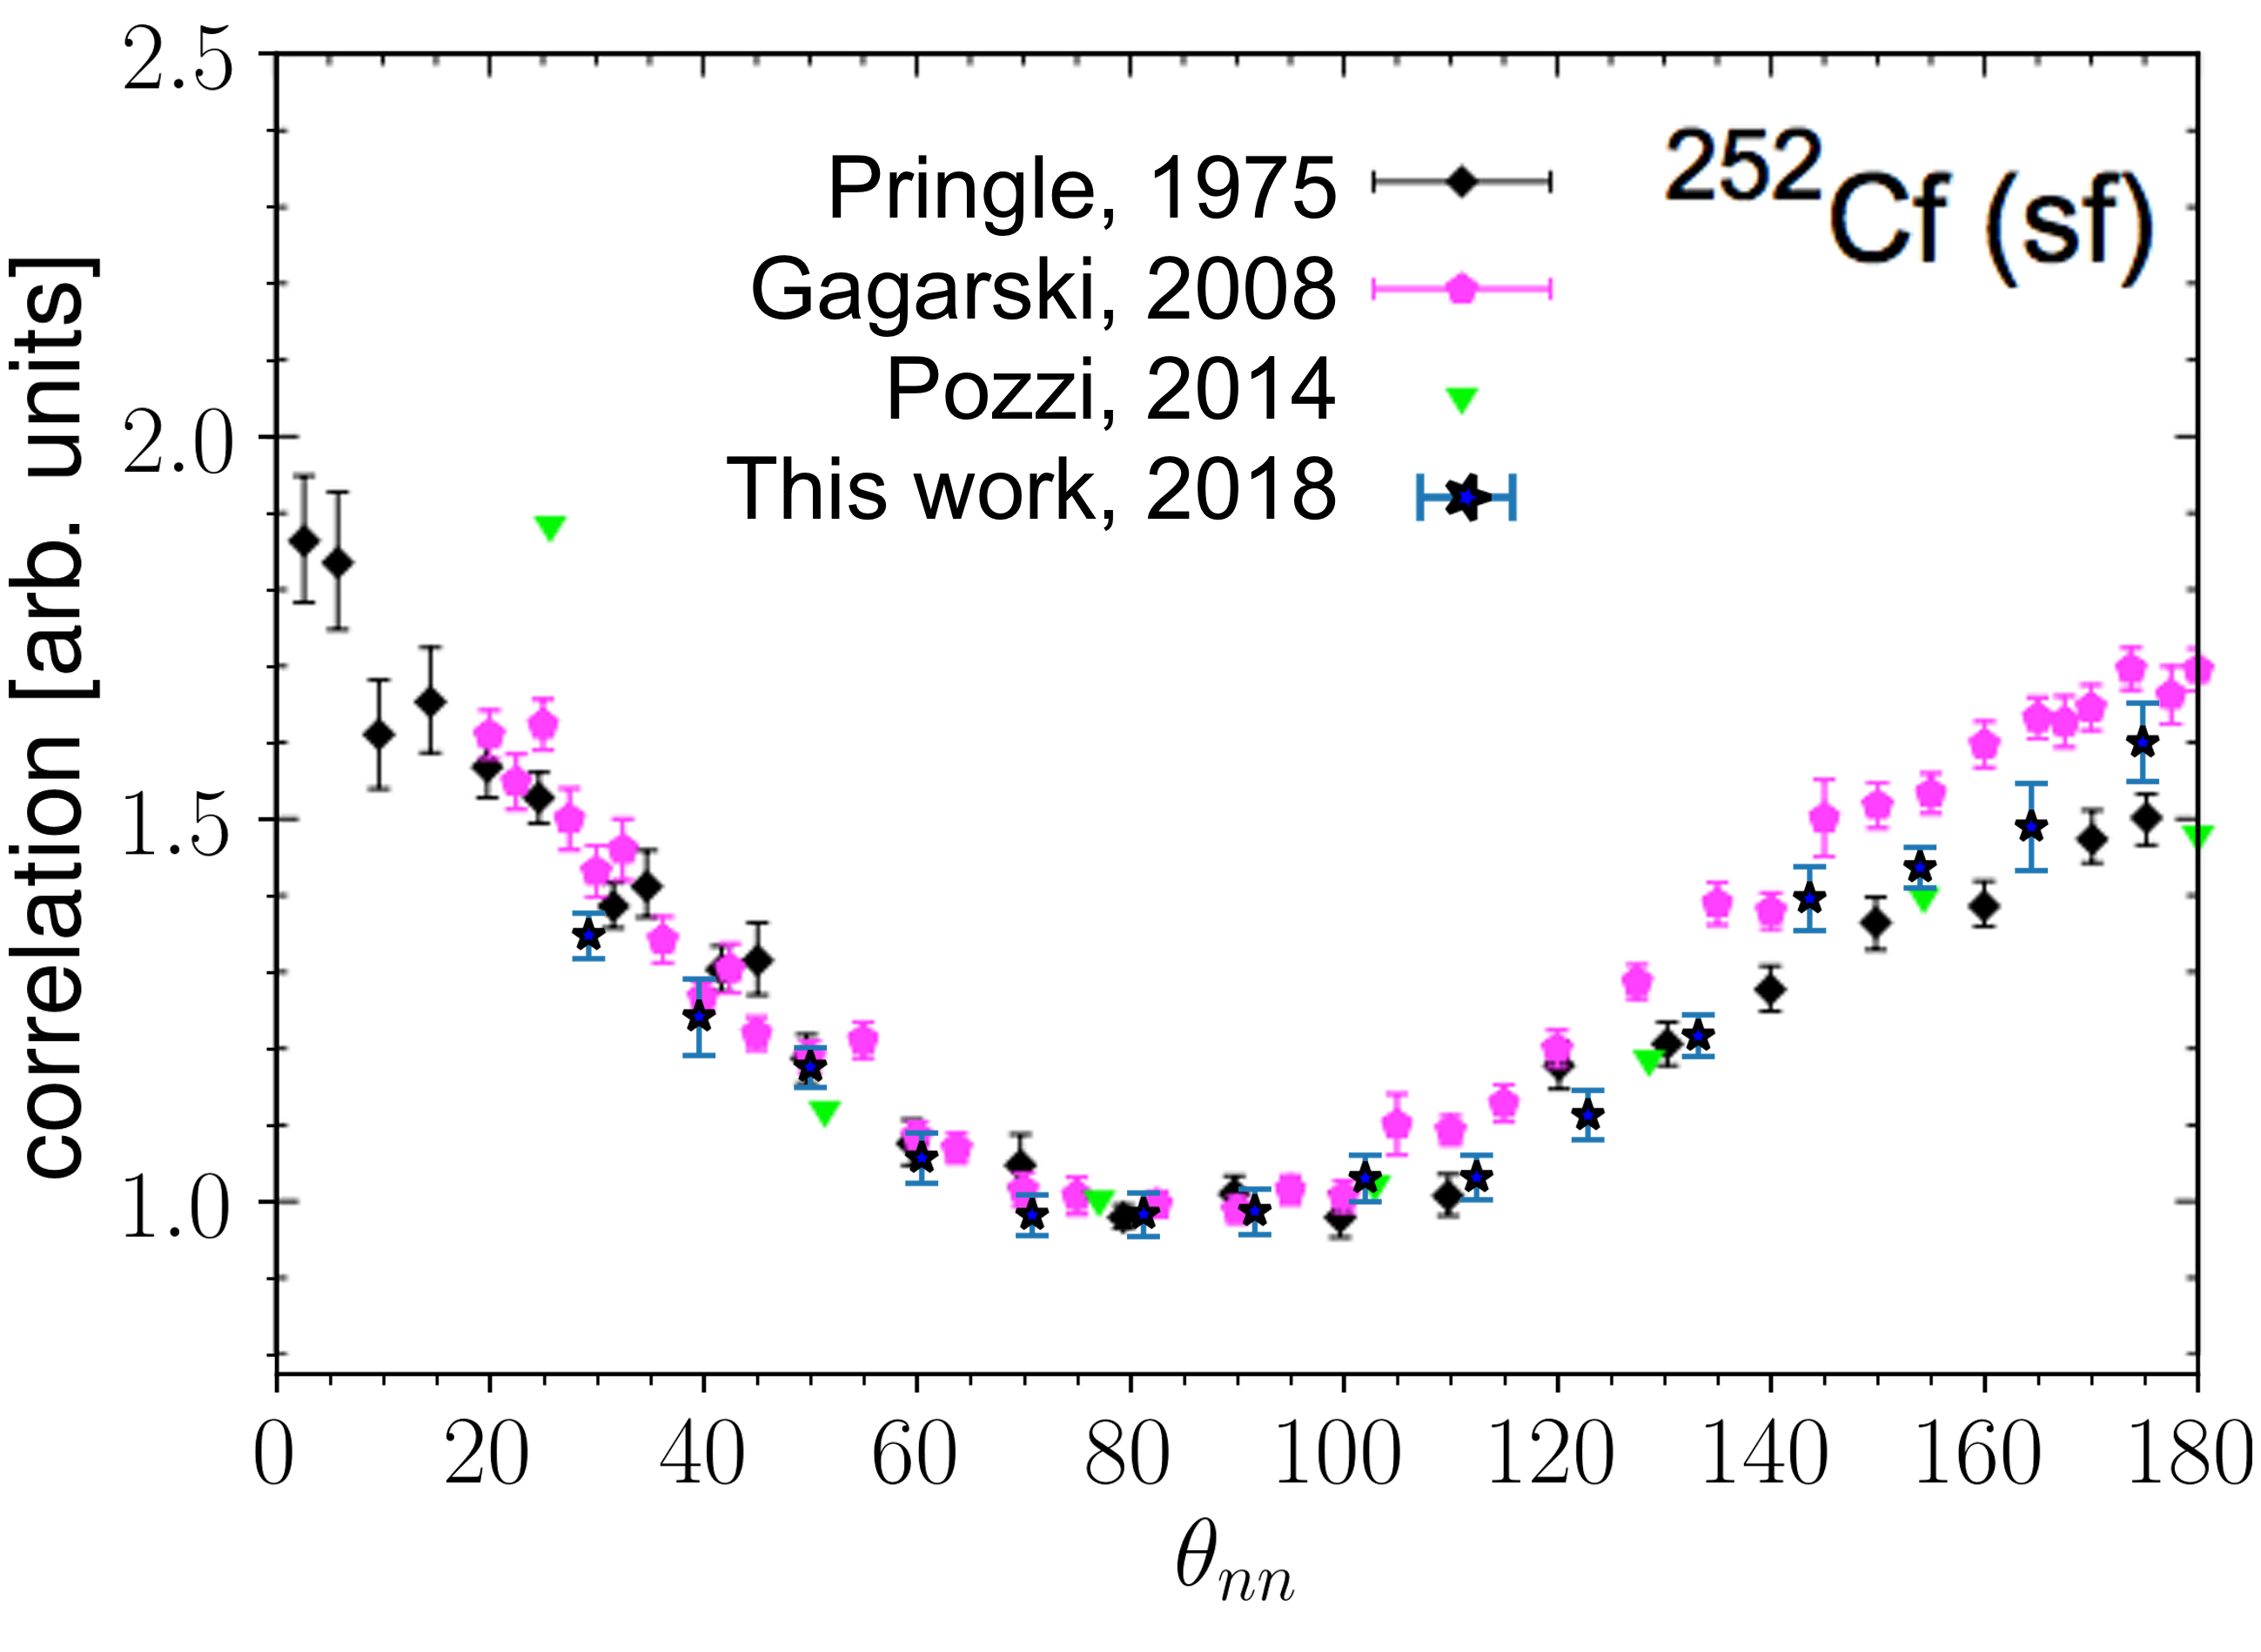
\includegraphics[width=0.7\textwidth]{Content/Introduction/Cf252_us_vs_them.png}
\caption{$\theta_{nn}$ distribution from the SF of $^{252}$Cf.
 The neutron detection threshold for Pringle~\cite{1975Cf252}, Gagarski~\cite{2008CF252}, and Pozzi~\cite{Pozzi2016} is 0.425 MeV, 0.425 MeV, and 0.7 MeV, respectively, and for this work is 0.5 MeV.
}
\label{fig:Cf252_us_vs_them}
\end{figure}
